\clearpage
\section{Additional plots for the analysis}

\subsection{TFR}

\begin{figure}[htbp]
	\centering
	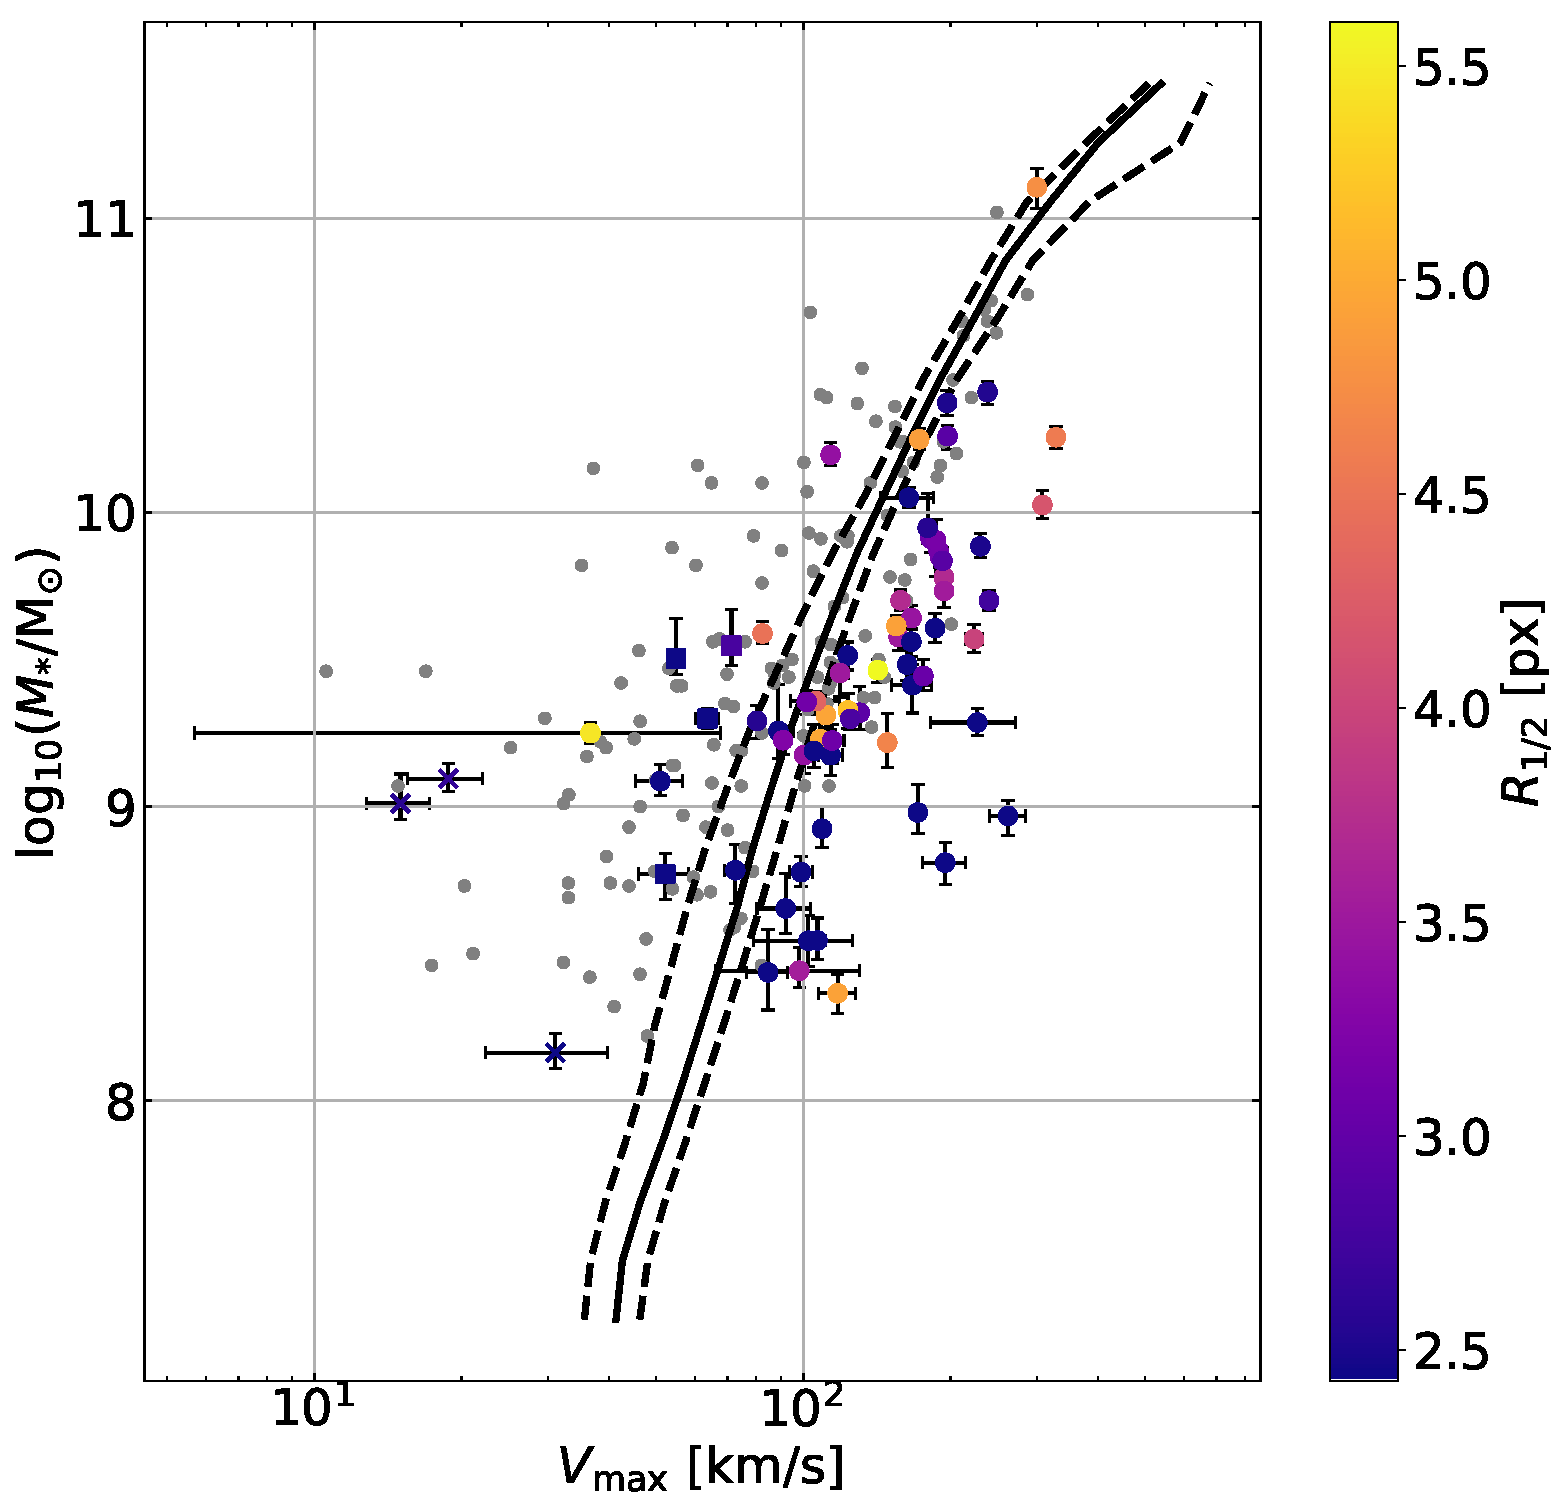
\includegraphics[width=\linewidth]{{../Plots/TFR_sizePX}.pdf}
	\caption[TFR as a function of angular size]{Same plot as in Fig.\,\ref{fig:TFR} but colour coded according to the apparent angular size (half-light radius) on the sky. The legend is similar to that in Fig.\,\ref{fig:TFR}. As for redshift, we do not find a significant evolution, though all the dispersion dominated galaxies with low $V_{\rm{max}}$ are also found to have the lowest sizes, which is in agreement with the results shown in Fig.\,\ref{fig:V_sgima_size}.}
	\label{fig:TFR_sizePX}
\end{figure}



\newpage
\subsection{Effect of the inclination on the TFR}
\begin{figure}[htbp]
	\centering
	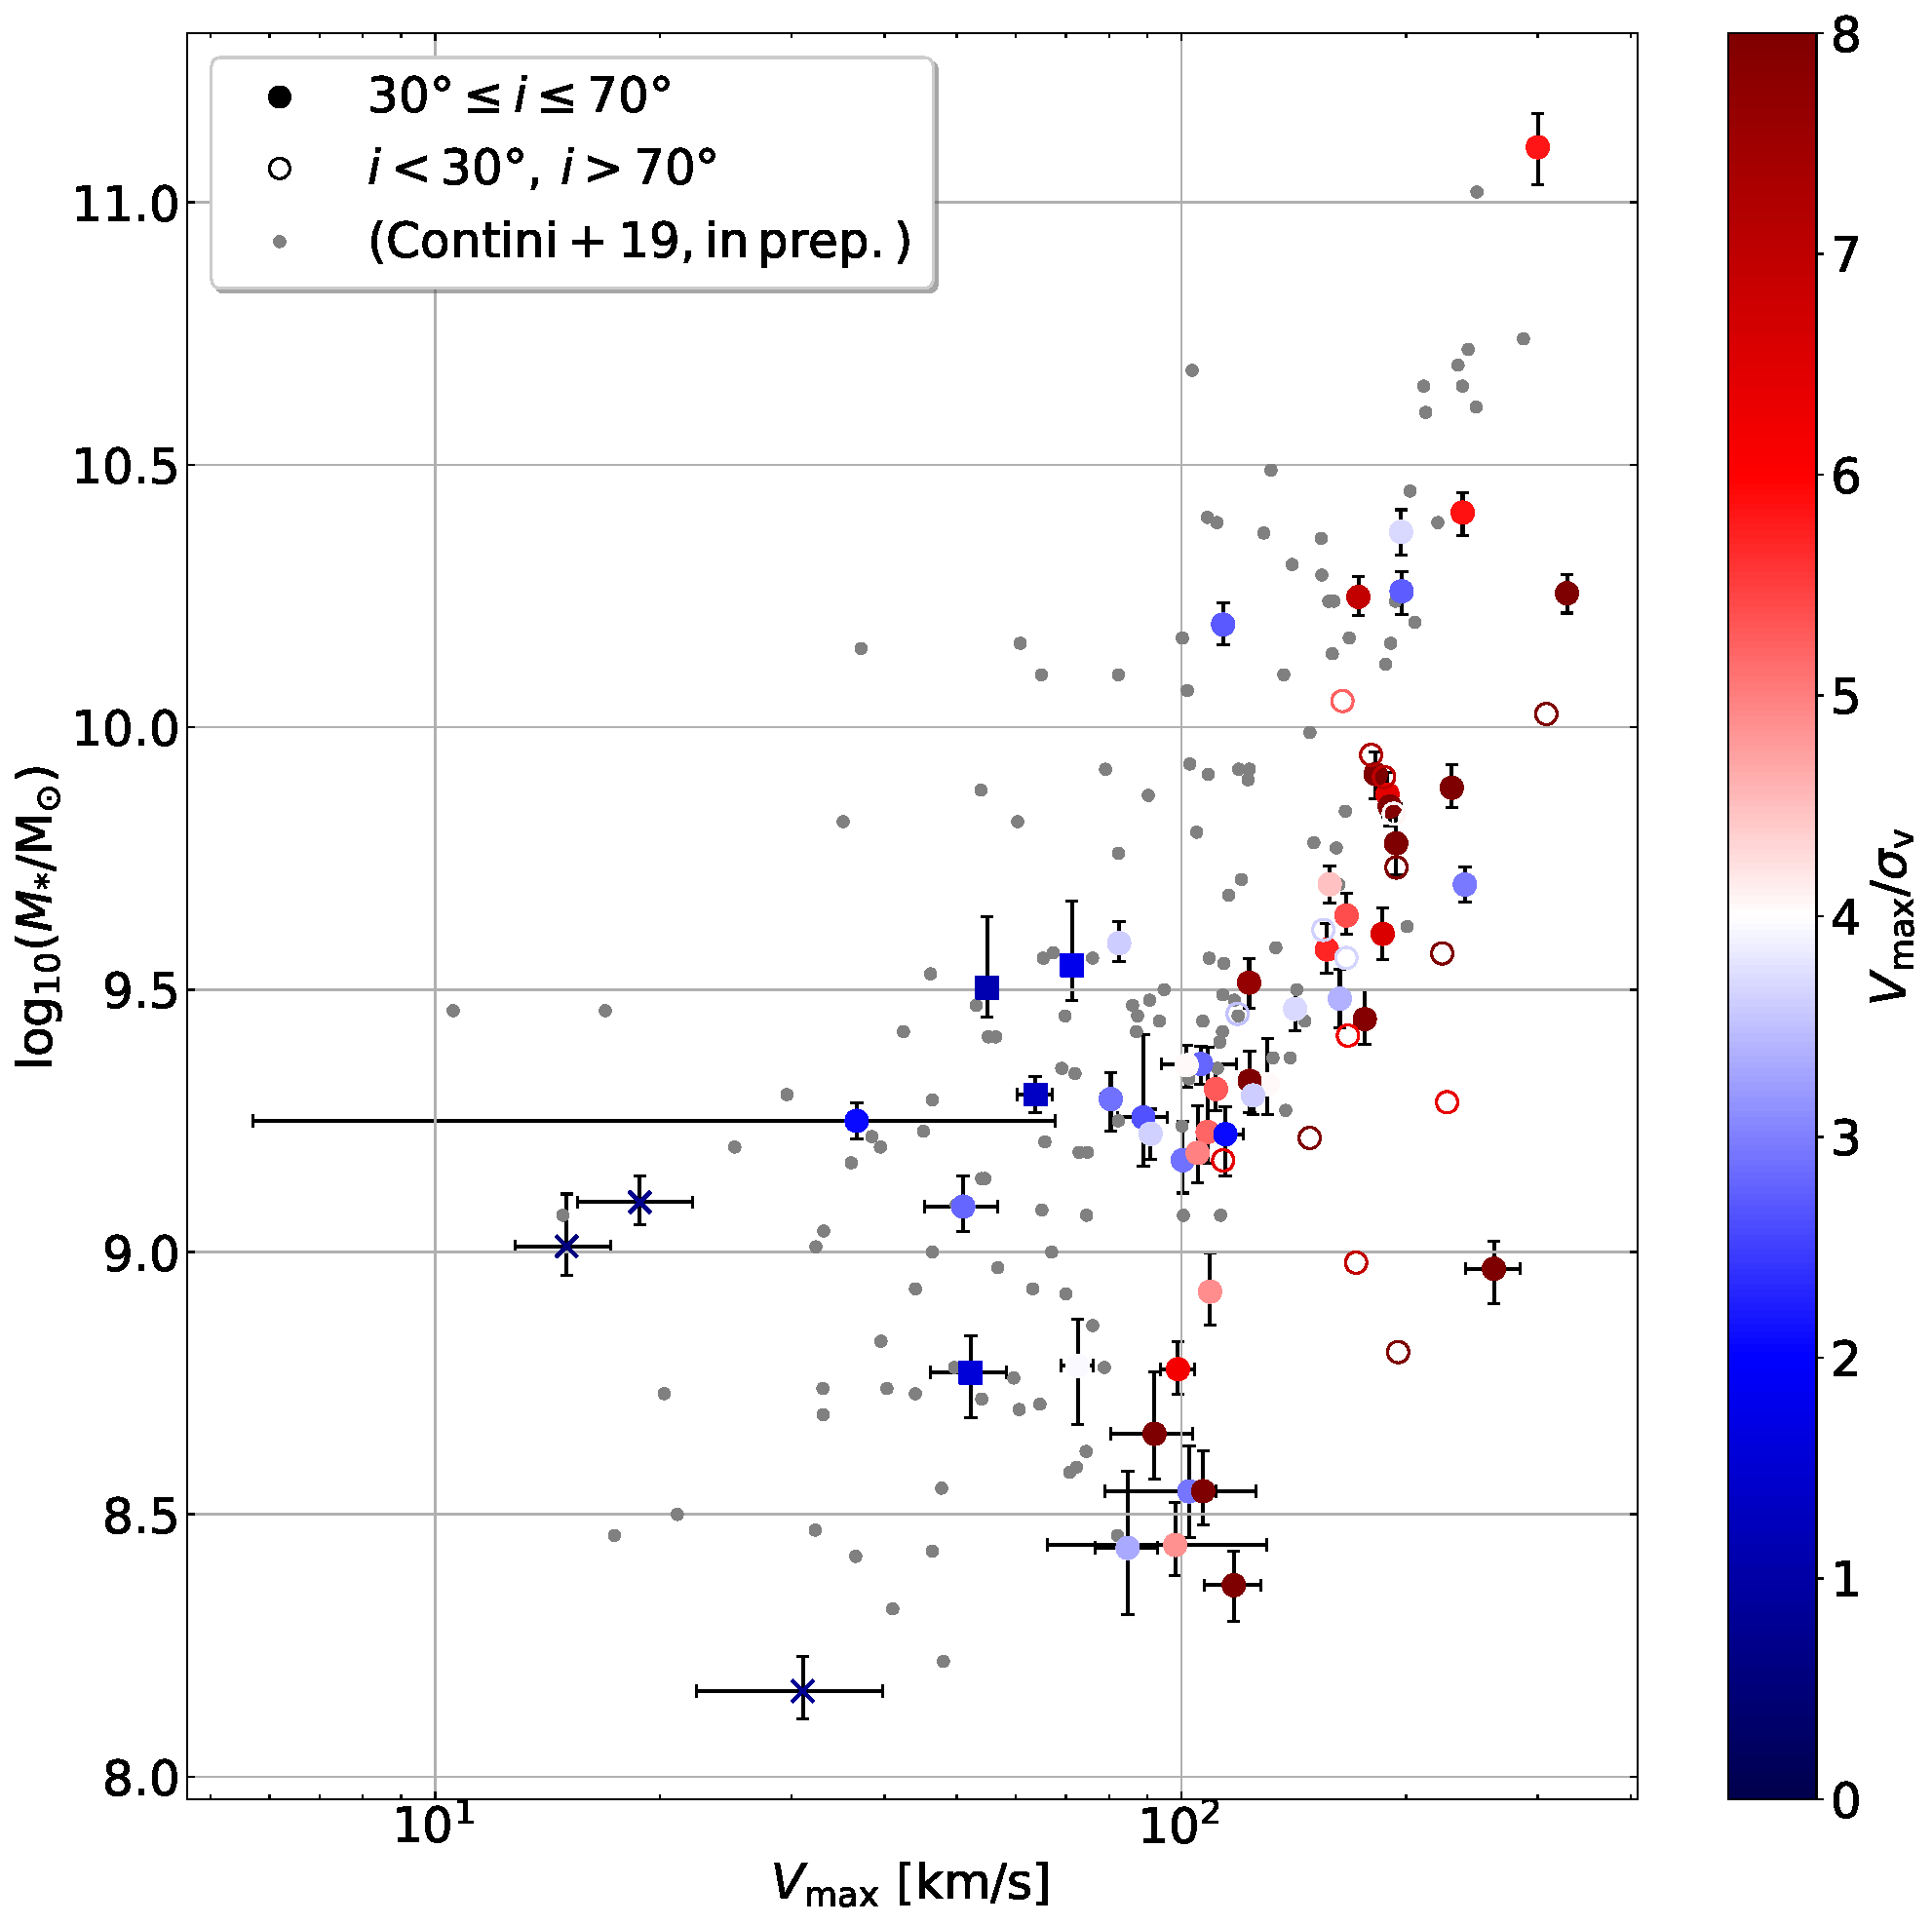
\includegraphics[width=\linewidth]{{../Plots/TFR_vel_corrected_of_i}.pdf}
	\caption[Effect of the inclination on the TFR]{Tully-Fisher Relation for galaxies with a reasonable inclination $30\degree \leq i \leq 70\degree$ (filled circles with error bars) compared against face-on ($i<30\degree$) and edge-on ($i>70\degree$) galaxies.}
	\label{fig:TFR_inc}
\end{figure}



\newpage
\subsection{$\rm{SFR} - V_{\rm{max}}$ relation}
\begin{figure}[htbp]
	\centering
	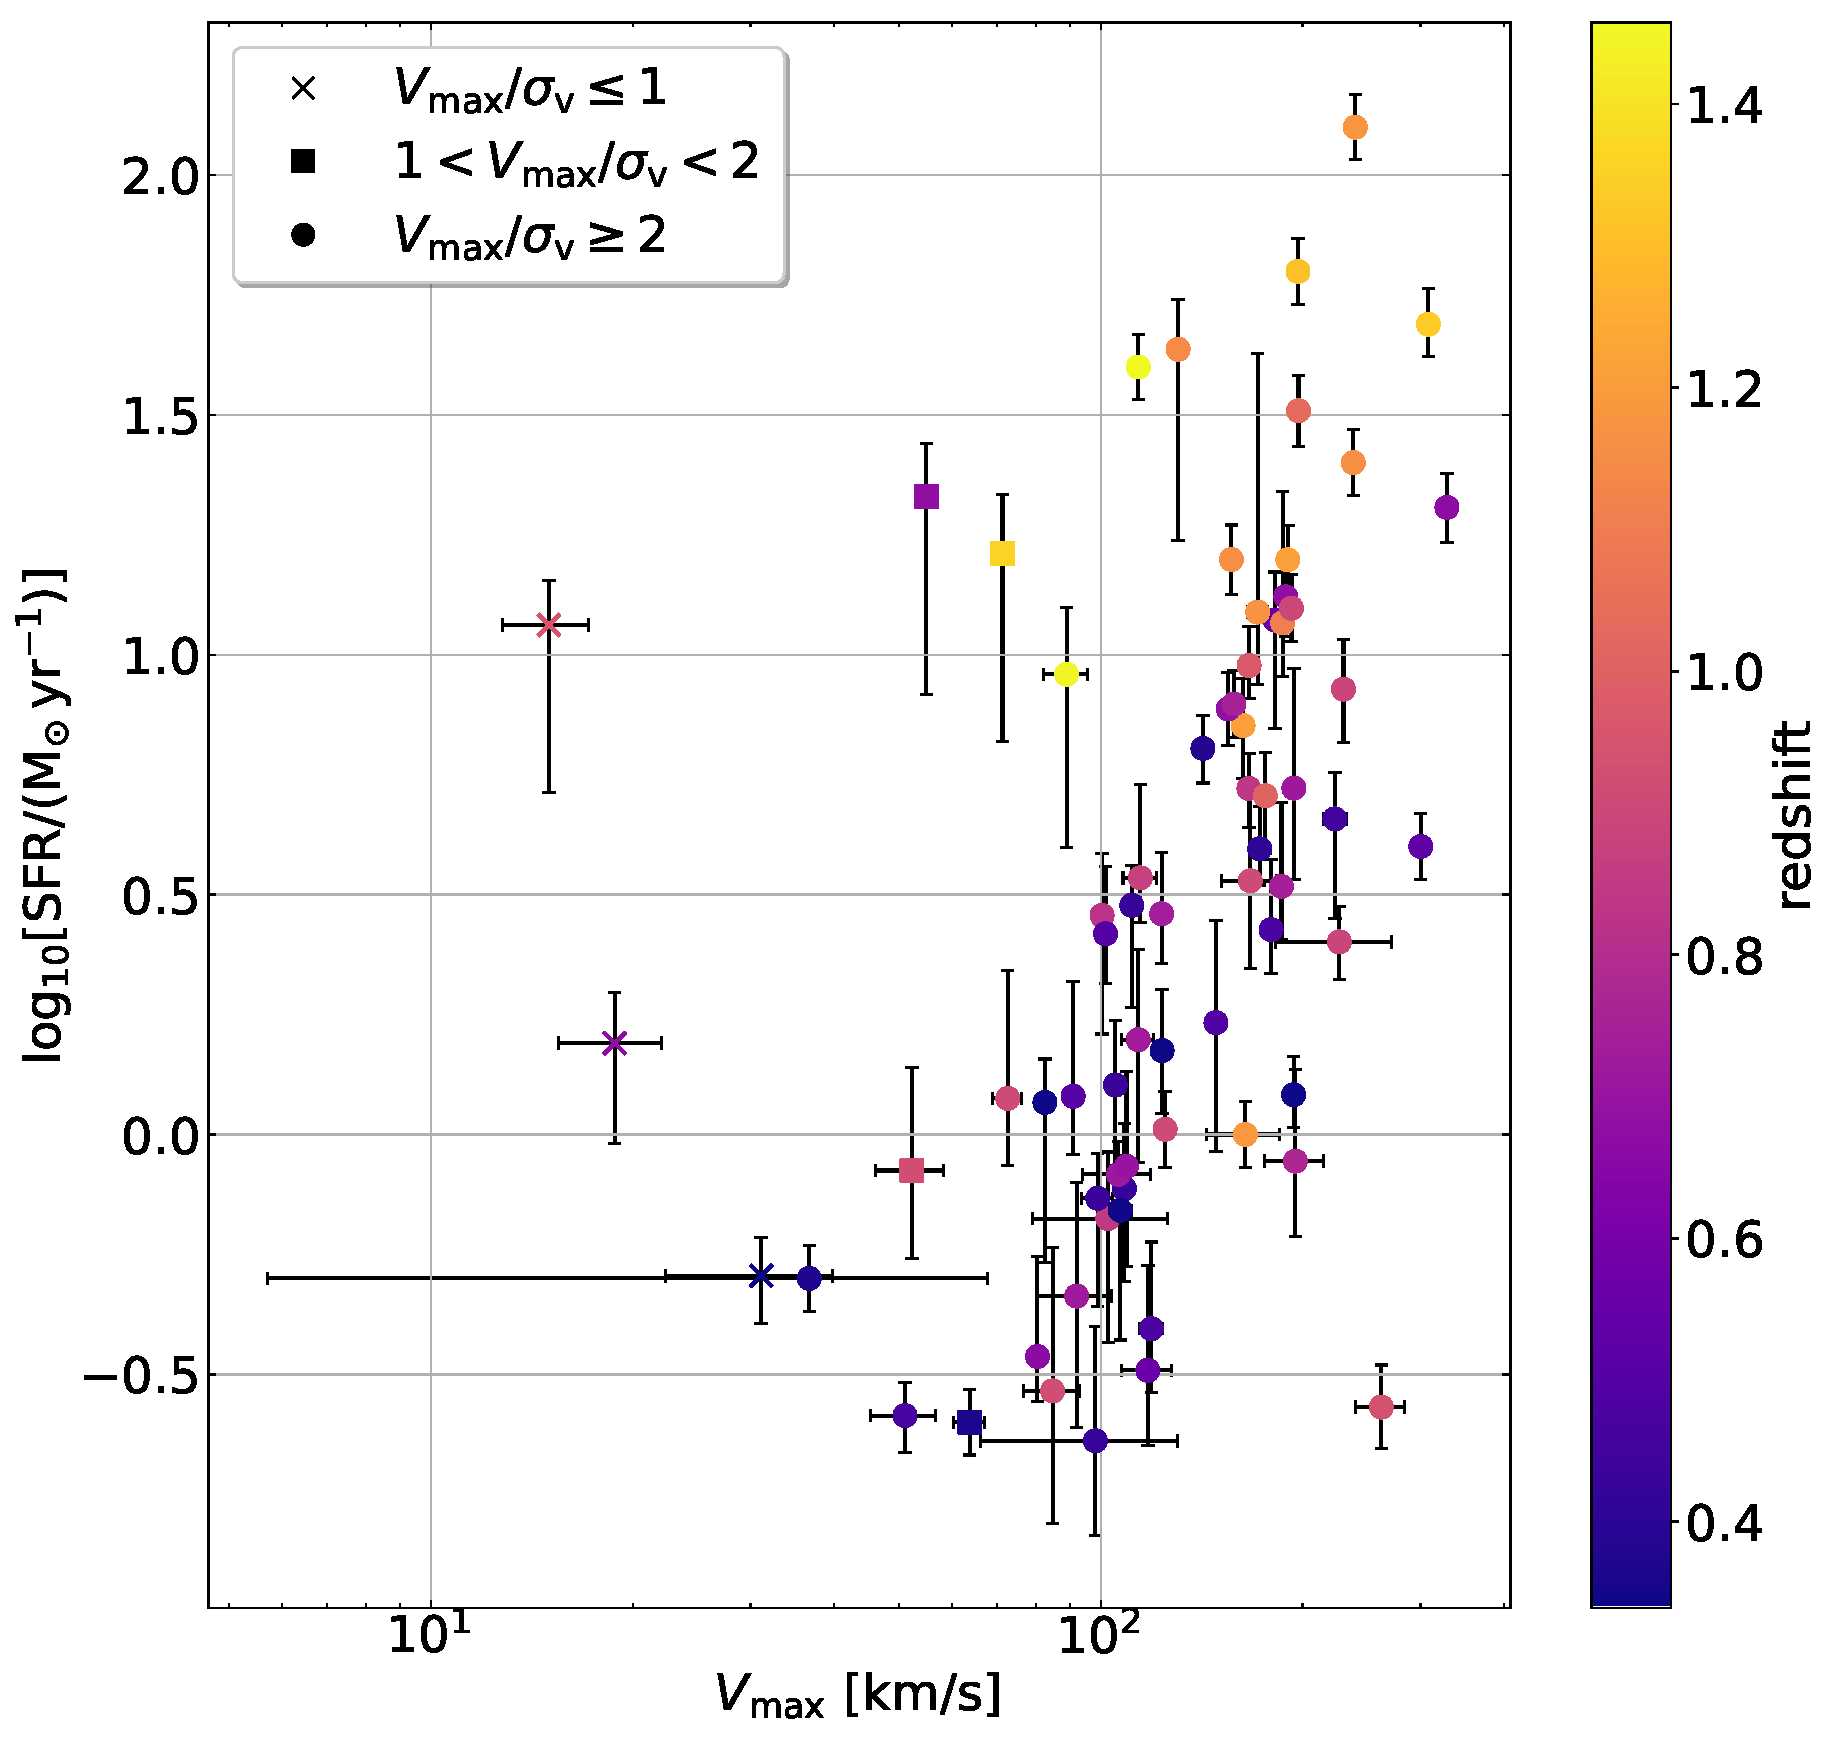
\includegraphics[width=\linewidth]{{../Plots/SFR_Vmax}.pdf}
	\caption[$\rm{SFR} - V_{\rm{max}}$ relation]{$\log_{10} \rm{SFR} - \log_{10} V_{\rm{max}}$ diagram with galaxies colour coded according to their redshift. We find a link between the $\rm{SFR}$ and the maximum rotation velocity. This is consistent with the galaxies main-sequence shown in Fig.\,\ref{fig:sfr_vs_mass} and with the TFR in Fig.\,\ref{fig:TFR}. }
	\label{fig:SFR_Vmax}
\end{figure}